
The general equation of a circle is 
\begin{align}
\implies \vec{x}^T\vec{x} - 2\vec{O}^T\vec{x} + \norm{\vec{O}}^2 - r^2  &= 0 \label{eq:converted_circle_examp}
\end{align}

Comparing equation \eqref{eq:converted_circle_examp} with the given circle equation:
\begin{align}
\vec{O} &= \myvec{-4\\-5}\\
\norm{\vec{O}}^2 &= 41 \\
r^2 &= 41 + 8 \\
\therefore r &= 7
\end{align}

The following Python code generates Fig. \ref{fig:4.2.2_circle2_circle_examp}

\begin{lstlisting}
solutions/2/codes/circle_exam.py
\end{lstlisting}
 
\begin{figure}[!ht]
\centering
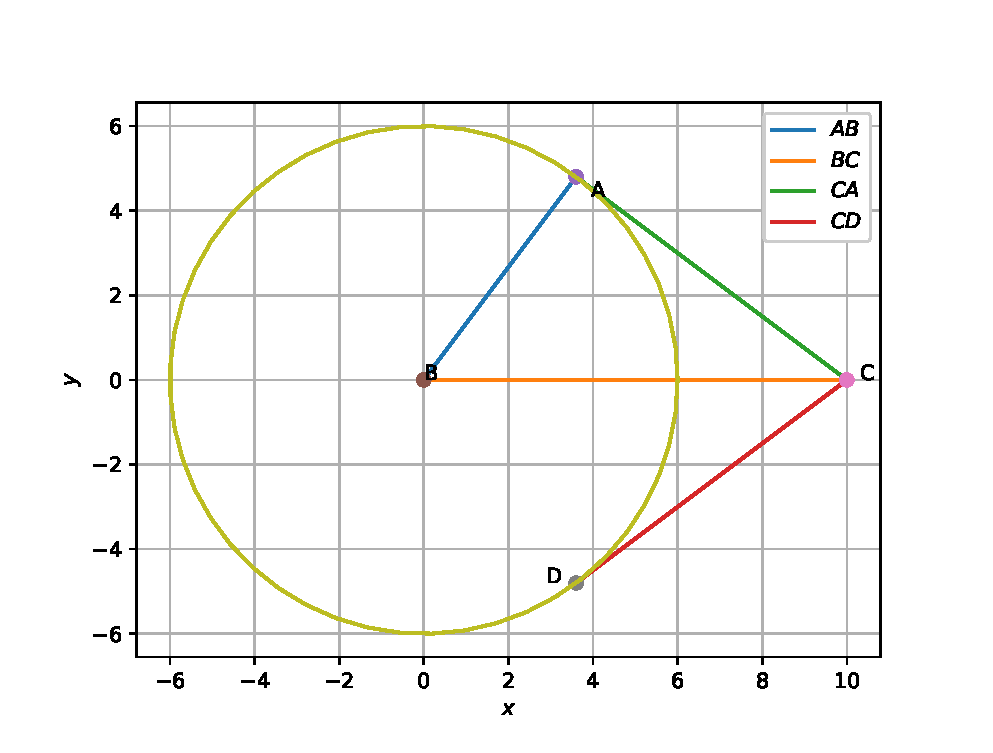
\includegraphics[width=\columnwidth]{./solutions/2/figs/circle_examp/circle.eps}
\caption{}
\label{fig:4.2.2_circle2_circle_examp}
\end{figure} 


